See  
\figref{fig:chapters/10/7/4/6Fig1}.
\begin{figure}[!h]
 \begin{center}
 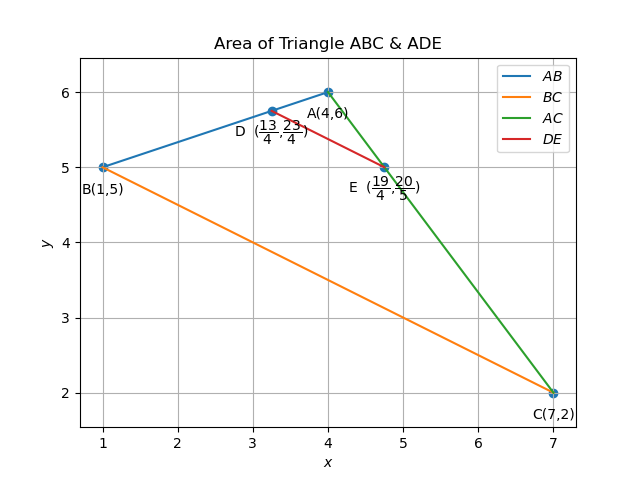
\includegraphics[width=\columnwidth]{chapters/10/7/4/6/figs/fig.png}
 \end{center}
\caption{}
\label{fig:chapters/10/7/4/6Fig1}
\end{figure}
	Using section formula
	  \eqref{eq:section_formula},
\begin{align}
\vec{D} =\frac{3\vec{A}+\vec{B}}{4}
	=\frac{1}{4}\myvec{13\\ 23}
	\\
\vec{E} =\frac{3\vec{A}+\vec{C}}{4}
	=\frac{1}{4}\myvec{19\\ 20}
	\\
	\vec{A}- \vec{D} 
	=\frac{1}{4}\myvec{3\\ 1},\,
	  \vec{A}- \vec{E}  
	=\frac{1}{4}\myvec{-3\\ 1}
	\\
	\vec{A}- \vec{B} =\myvec{3\\1},
	  \vec{B}-\vec{C} =\myvec{-6\\3}
	  \\
\implies	ar(ABD) =\frac{1}{2} \norm{\brak{\vec{A}-\vec{D}}  \times 
   \brak{\vec{A}- \vec{E}}} 
	=	\frac{15}{32}
	\\
	  ar(ABC) =\frac{1}{2} \norm{\brak{\vec{A}-\vec{B}}  \times 
   \brak{\vec{B}- \vec{C}}} 
	=	\frac{15}{2}
	\\
	\implies \frac{ar\brak{ADE}}{ar\brak{ABC}}=\frac{1}{16}
\end{align}
